\documentclass[12pt,a4paper]{article}
\usepackage[utf8]{inputenc}
\usepackage{amsmath}
\usepackage{amsfonts}
\usepackage{amssymb}
\usepackage{graphicx}
\usepackage{hyperref}
\usepackage[margin=0.5in]{geometry}

\graphicspath{ {./images/} }
\author{Oleg Loshkin}
\title{Simple Online FPS}

\hypersetup{
    colorlinks=true,
    linkcolor=blue,
    filecolor=magenta,      
    urlcolor=cyan,
}

\begin{document}

\maketitle

\section{Introduction}
This game is the result of the \textbf{SAE's repeat session for the GPR5100 Game Networking module}. \textbf{The aim of this project was to make a simple but functional online game} using Unity and a networking technology of our choice.

\section{Technologies used}
\begin{itemize}
\item \textbf{Unity 2018.4.9f1:}\\
Latest available LTS version of Unity available at the time the project had started.
\item \textbf{Photon Bolt:}\\
High level game networking API for Unity. \textbf{The API provides some features that match perfectly the requirements of an online FPS}, namely lag compensating hitboxes and raycasting which negates the need to implement this complex feature manually.
\item \textbf{Github:}\\
Github was used for versioning. \textbf{The project's repository is available \href{https://github.com/LoshkinOleg/NetworkingRattrapage}{here}} .\\
The repository was temporarely split between two branches mid project to explore a possible migration to Photon Pun. This idea was abandonned and game was implemented using Photon Bolt.
\end{itemize}

\section{Gameplay}
\begin{center}
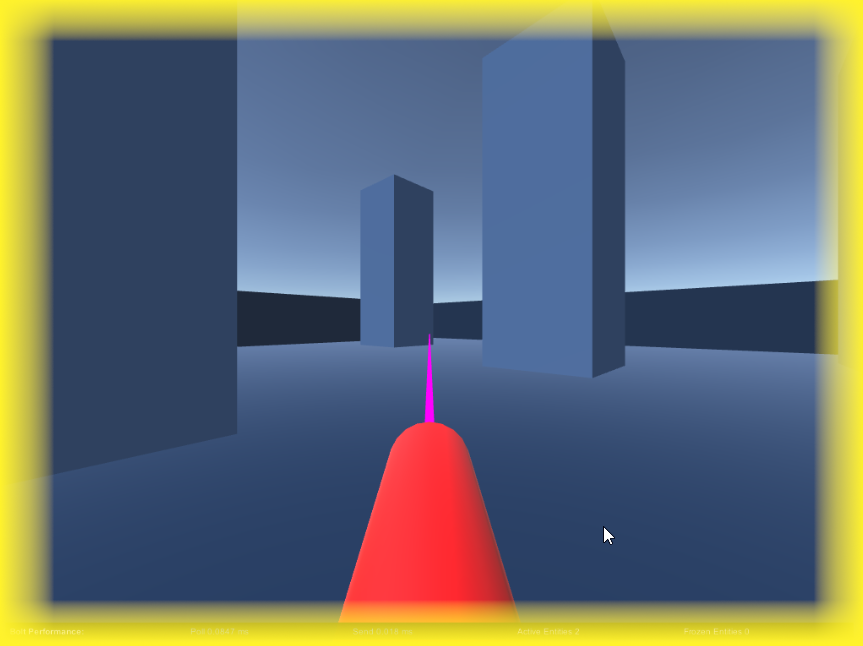
\includegraphics[scale=0.75]{gameplay}
\end{center}
\begin{itemize}
\item \textbf{The Lobby:}\\
The player can either \textbf{create a new game session} and name it \textbf{or join a random game session currently in progress}. Upon the creation of a session, the host joins it as a listen server.\\
Note that the session's name is currently unused as no list of sessions is visible anywhere, that sessions cannot be password protected and the number of maximum players per session cannot be established.
\item \textbf{The Arena:}\\
The arena is a \textbf{square area surrounded by walls and dotted with pillars that server as cover}. \textbf{Spawn points are located on the outer periphery of the arena close to the pillars}.
\item \textbf{The Controls:}\\
Players can \textbf{shoot with Left Mouse Button}, \textbf{look around horizontally only using the mouse} and \textbf{move around using WASD keys}.
\item \textbf{The Fight:}\\
\textbf{A 2 second cooldown is enforced between each shot} a player takes. \textbf{A player can take two hits from an adversary before dying}. No ways to regenerate health exist. \textbf{Upon death, the player respawns at the spawn point furthest away from the average position of all other players}.
\newpage
\item \textbf{The Feedbacks:}\\
\begin{itemize}
\item A \textbf{shooting sound} is played upon any shot.
\item A \textbf{reloading sound} is played just before the end of the shooting cooldown and \textbf{the sound's end indicates the end of the cooldown}. Only the local player hears this sound.
\item \textbf{Getting hit} triggers a \textbf{grunting} sound from the player. Only the player being hit hears this sound.
\item \textbf{Upon landing a shot} on a player, \textbf{a ringing sound is played} for every player except the one being hit.
\item Upon \textbf{being hit once}, the player's \textbf{screen edges turn yellow}. \textbf{Being hit a second time} turns the \textbf{edges turn red}. A third hit kills the player and the health indicating overlay resets.
\end{itemize}
\end{itemize}

\section{Movement}
The movement in the game is \textbf{client authoritative} and uses \textbf{interpolation}. It is implemented using \textbf{Photon Bolt's Transform State and Commands}. While using RigidBodies is impossible in conjunction with Photon Bolt, Unity's "Character Controller" component has provided a good replacement for movement and collisions.\\\\
Client authoritativity not being ideal in online FPS games, a server authoritative movement was originally planned. However, after much efforts trying to make it work, Photon Bolt's rollback and lack of documentation of it's inner workings has made this idea too difficult to execute.

\section{Hitscanning}
Implementation of hitscanning was surprisingly easy using \textbf{Photon Bolt's Hitboxes and it's BoltNetwork.RaycastAll() method}. The only caveats that had to be worked around was the inability to filter the targets and the fact that the raycast does not interact with non-Bolt game objects like walls.
\newpage

\section{Lobby}
\begin{center}
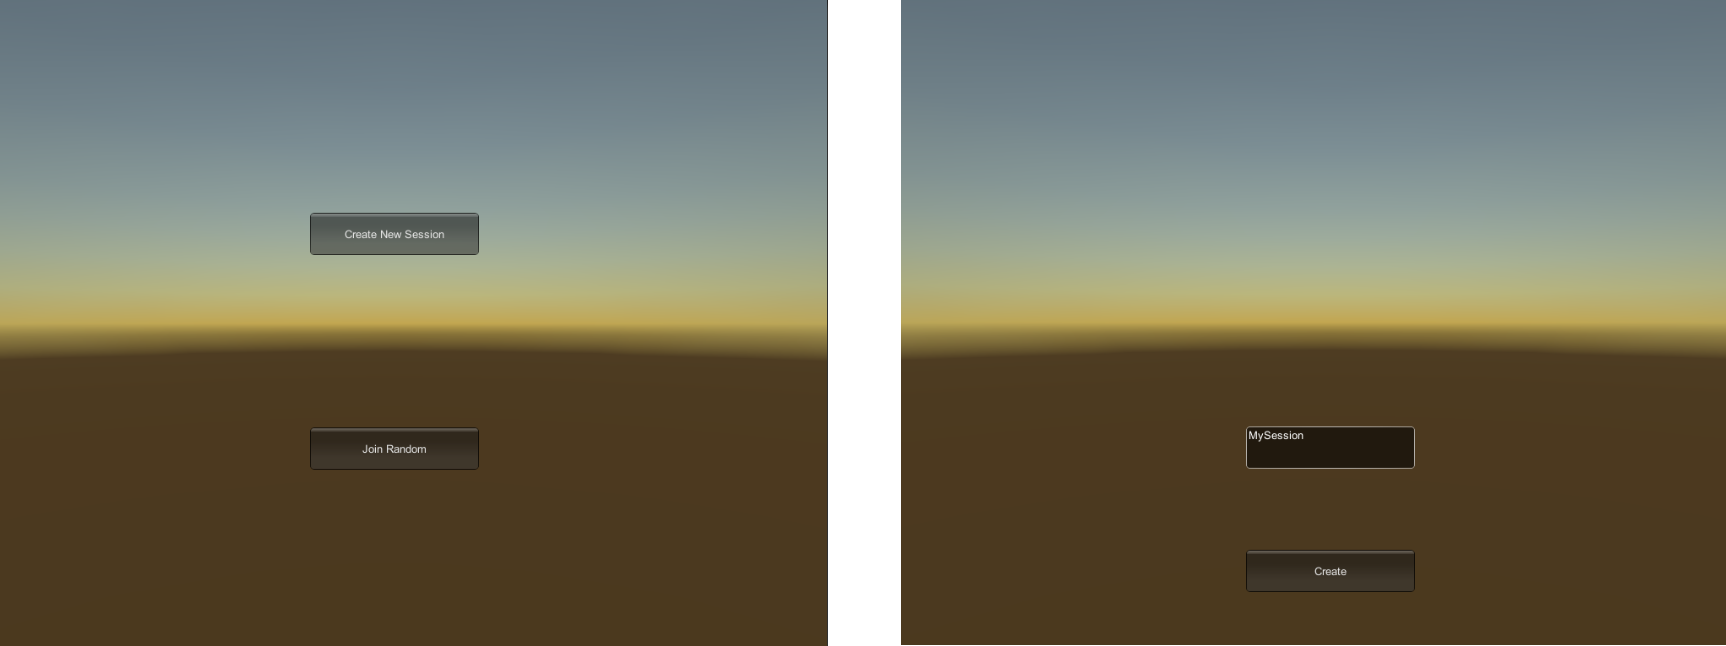
\includegraphics[scale=0.4]{lobby}
\end{center}
The lobby is comprised of \textbf{two tabs}: a main one with two buttons for \textbf{creating a new session or to join a random one}, and \textbf{a tab for naming the new session before joining it}.\\
A different lobby was originally planned, one that would display a list of all current game sessions in progress with their name, the number of players and whether or not they are protected by a password. This could not be implemented for the following reasons:\\\\
Photon Bolt provides a static property under "BoltNetwork.Sessions" to allow the program to retrieve all ongoing sessions. However, this list of sessions is unexplicablely always empty. The idea of displaying a list of ongoing sessions had therefore to be abandoned.\\
Instead, Photon Bolt's BoltMatchmaking.JoinRandom() static method is used to join any ongoing game session, bypassing the sessions list completely and successfully finding any existing sessions.\\\\
A password protection and maximal number of players per session limit was not implemented either: while the documentation of Photon Bolt goes to length about the usage of it's BoltMatchmaking utility class, it does not provide any concrete examples of implementations of password protection and the documentation does not provide any explicit enough ways to handle session customization.\\\\
For these reasons, the lobby is as minimalistic as it is.

\section{Feedback}
Feedbacks for the gameplay have been implemented using \textbf{Photon Bolt's Events}. This allows the various feedbacks to be played on the programs of all players in a session when needed.\\
Albeit functional, these are still bug prone due to my lack of understanding of the Photon Bolt's API and the way it handles event sending and reception depending on the various confusing configurations that can be used.

\section{Potential Improvements}
\begin{itemize}
\item Clicking "Join Random" in the lobby without any running sessions locks the client into an indefinite state where they can't do anything and that they cannot escape without restarting the game. This is due to the bug described in the Lobby section that prevents the implementation of a check to verify the non existence of any sessions.
\item The visual aspect of the game was completely neglected. Any assetwork would improve the player's experience.
\item While the player can name a session when creating one, due to the above mentioned "BoltNetwork.Sessions" bug, no session list are displayed in the lobby and the name given by the player upon session creation is not used in any way.
\item There are no kill to death ratio counters.
\item The game does not perform any checks to verify that the session in progress is not playable (eg: less than 2 players in session).
\item Sessions cannot currently be protected by a password.
\item The host cannot define a limit on the number of players allowed in a session.
\item Bots for testing the game's reaction to lag would have been a good addition to the project (eg. zigzagging, peeking from around corner, etc.).
\item Having more than two players in a session creates auditive bugs due to the way network events are handled.
\end{itemize}

\section{Summary}
\textbf{The game fulfils it's basic ambitions}: \textbf{it is a barebone online FPS that successfully synchronizes players and performs hitscans for firing.}\\\\
Photon Bolt has proven very difficult to work with. Each new feature, however simple and small it may be required hours of debugging.\\
During the development, I've encountered bugs due to possibly inner workings of the API that rendered impossible the implementation of some key features, and weirder still, bugs coming from Unity's side that seemingly came from the interaction of Photon Bolt with the engine (eg: GameObject.FindGameOb\\jectWithTag() breaking).\\
All these holdbacks made me consider switching networking platforms but doing so would have meant discarding much of the work I had done up to that point.\\
Despite a somewhat complete documentation provided by Photon Bolt, I've found myself needing more to investigate these strange bugs but could not find any.\\
Moreover, I was unable to get help to overcome these issues due to my choice of Photon Bolt as the networking technology, my colleagues having picked different ones for their projects and the senior students and teachers being unfamiliar with the API.\\\\
Due to all of this, \textbf{the game's current status is lacking in both features and polish} and I am left to wonder how much of the problems encountered have it's origin in my own abilities and how much in the framework's choice.

\end{document}